\section{Results}
\label{sec:results}

\subsection{Human and \llm Spatial Texts Are Highly Separable}
\label{sec:classification-results}

\begin{table}[t]
    \centering
    \resizebox{\textwidth}{!}{%
    \begin{tabular}{@{}llcccc@{}}
        \toprule
        \textbf{Scope} & \textbf{Feature family} & \textbf{Accuracy} & \textbf{F1} & \textbf{ROC-AUC} & \textbf{95\% acc. CI} \\
        \midrule
        All & Length-only & 87.7 & 89.0 & 90.9 & 83.3--92.5 \\
        All & Spatial-only & 87.7 & 88.4 & 95.6 & 85.9--89.1 \\
        All & Narrative-only & 94.7 & 94.8 & 97.8 & 92.6--96.5 \\
        All & All without length & 96.5 & 96.6 & 98.3 & 94.7--98.7 \\
        All & All features & {\bf 97.4} & {\bf 97.4} & {\bf 99.7} & {\bf 95.1--99.1} \\
        \midrule
        \rtr & Spatial-only & 98.1 & 98.2 & 100.0 & 95.6--100.0 \\
        \rtr & All without length & {\bf 100.0} & {\bf 100.0} & {\bf 100.0} & {\bf 100.0--100.0} \\
        \midrule
        \writingprompts & Length-only & 69.1 & 69.6 & 82.0 & 60.9--75.3 \\
        \writingprompts & Spatial-only & 83.8 & 84.1 & 89.1 & 72.9--95.7 \\
        \writingprompts & All without length & 94.1 & 94.3 & 95.8 & 92.5--97.1 \\
        \writingprompts & All features & {\bf 95.6} & {\bf 95.8} & {\bf 97.8} & {\bf 92.6--98.6} \\
        \bottomrule
    \end{tabular}}
    \caption{Author-classification results under stratified 5-fold cross-validation. Values are percentages. Best result within each scope is in \textbf{bold}.}
    \label{tab:classification}
\end{table}


\Figref{fig:classification-accuracy} and \tabref{tab:classification} show the main classifier results. Across the full corpus, all features reach 97.4\% accuracy and 99.7 ROC-AUC. Removing length barely changes the result: all non-length features still reach 96.5\% accuracy and 98.3 ROC-AUC. Spatial-only features reach 87.7\% accuracy, and the permutation test gives $p=0.0099$ for the spatial-only, all-without-length, and all-feature aggregate classifiers.

The source-specific results clarify the role of genre. In \rtr, all non-length features separate the two author classes perfectly, and spatial-only features reach 98.1\% accuracy. This is expected because human \rtr texts are route instructions while \gptmini outputs are first-person stories. The more important check is \writingprompts: length-only accuracy falls to 69.1\%, but spatial-only features still reach 83.8\%, all non-length features reach 94.1\%, and all features reach 95.6\%. This weakens the simplest explanation that the full-corpus result is only a route-instruction artifact.

\begin{figure}[t]
    \centering
    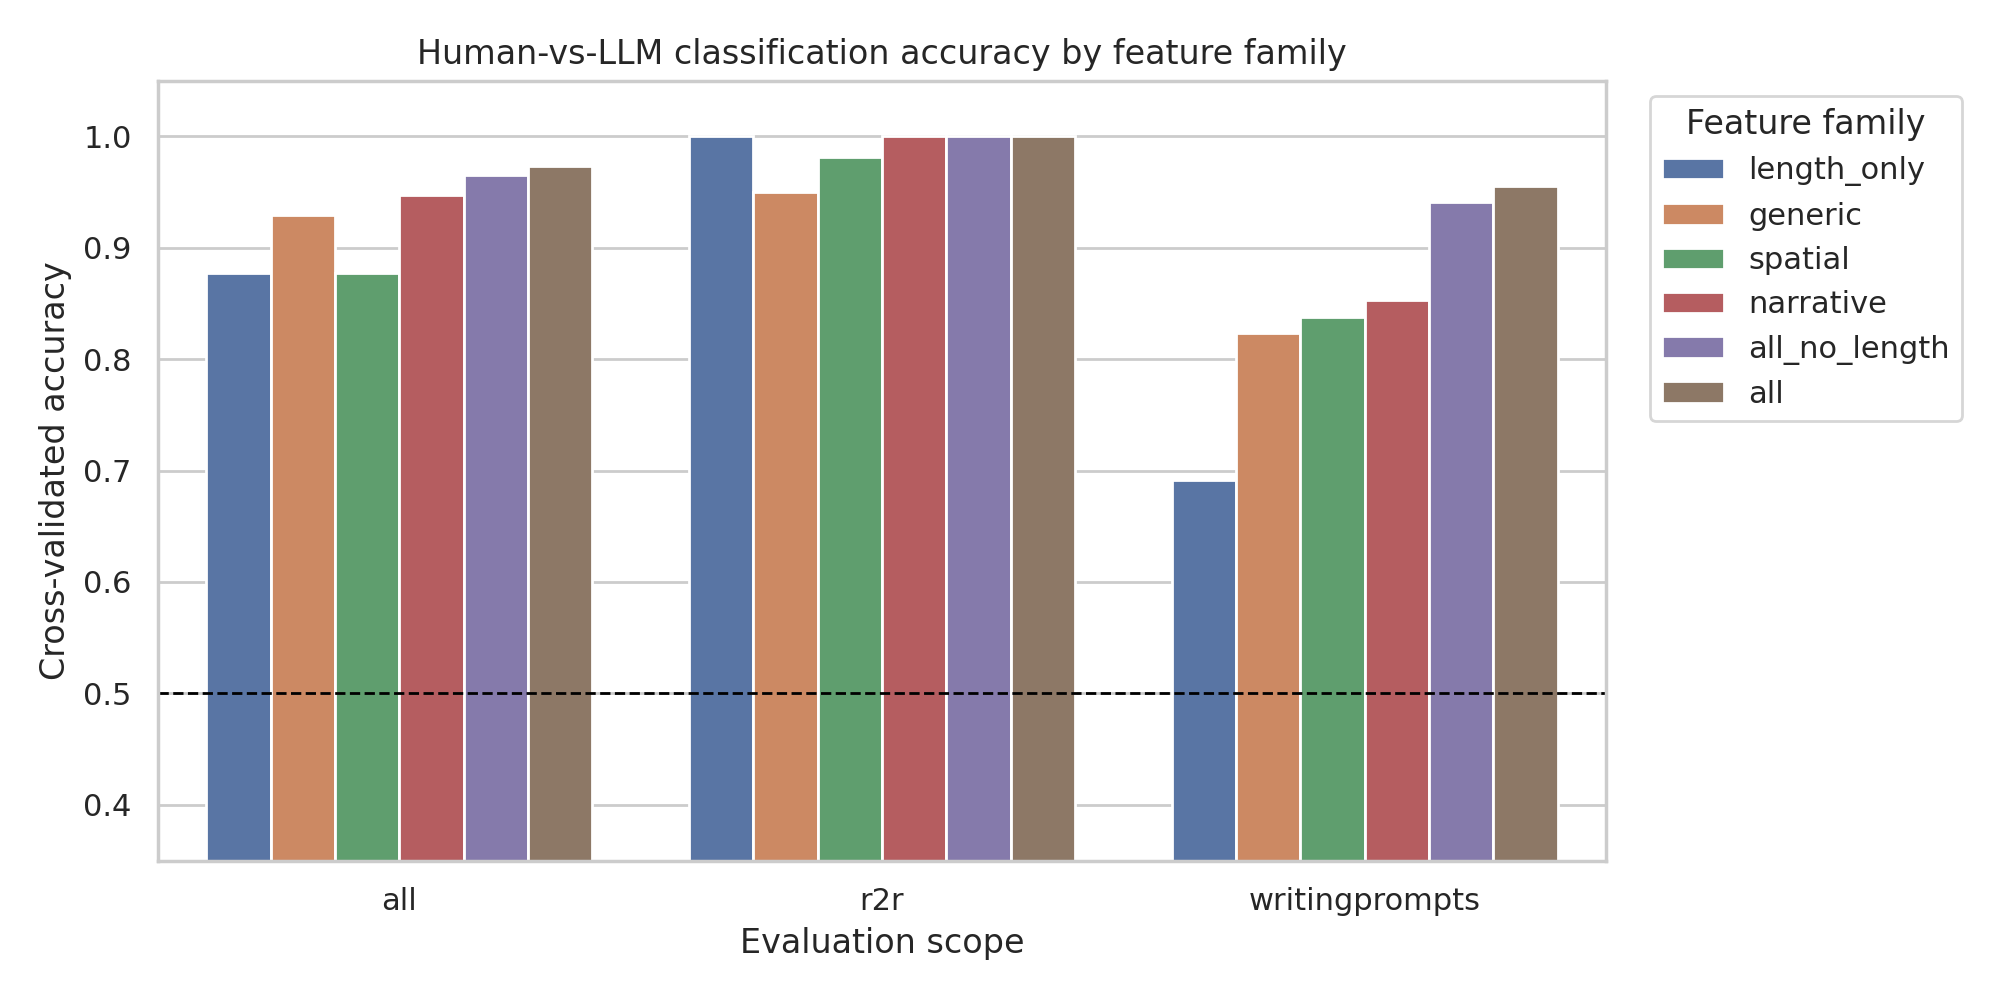
\includegraphics[width=0.95\linewidth]{figures/classification_accuracy.png}
    \caption{Classification accuracy by feature family. Spatial-only and narrative-only features both exceed the chance baseline, while all non-length features nearly match the full feature set.}
    \label{fig:classification-accuracy}
\end{figure}

\subsection{The \llm Profile Is Sensory, First-Person, and Landmark-Reusing}
\label{sec:feature-results}

\begin{table}[t]
    \centering
    \resizebox{\textwidth}{!}{%
    \begin{tabular}{@{}llrrlr@{}}
        \toprule
        \textbf{Scope} & \textbf{Feature} & \textbf{Human mean} & \textbf{\llm mean} & \textbf{Direction} & \textbf{BH $q$} \\
        \midrule
        All & \texttt{sensory\_per\_1000} & 1.77 & 14.67 & \llm higher & $5.41{\times}10^{-32}$ \\
        All & \texttt{formulaic\_phrase\_per\_1000} & 0.08 & 6.09 & \llm higher & $5.46{\times}10^{-30}$ \\
        All & \texttt{survey\_route\_ratio} & 0.252 & 0.065 & \llm lower & $5.09{\times}10^{-28}$ \\
        All & \texttt{imperative\_sentence\_share} & 0.543 & 0.000 & \llm lower & $1.50{\times}10^{-24}$ \\
        All & \texttt{first\_person\_per\_1000} & 20.53 & 74.21 & \llm higher & $1.62{\times}10^{-20}$ \\
        All & \texttt{landmark\_reuse\_ratio} & 0.121 & 0.317 & \llm higher & $1.03{\times}10^{-14}$ \\
        \bottomrule
    \end{tabular}}
    \caption{Key full-corpus feature differences after Benjamini-Hochberg correction. The largest effects show \gptmini using more sensory, formulaic, first-person, and landmark-reusing language, while human texts use more imperative route grammar.}
    \label{tab:key-features}
\end{table}


\Tabref{tab:key-features} lists the largest and most interpretable corrected feature differences. Across the full corpus, \gptmini uses far more sensory language than humans (14.67 vs. 1.77 terms per 1,000 tokens, BH $q=5.41{\times}10^{-32}$), more formulaic phrases (6.09 vs. 0.08 per 1,000, $q=5.46{\times}10^{-30}$), more first-person language (74.21 vs. 20.53 per 1,000, $q=1.62{\times}10^{-20}$), and more landmark reuse (0.317 vs. 0.121, $q=1.03{\times}10^{-14}$). Humans show higher imperative sentence share and higher survey/route ratio.

\begin{figure}[t]
    \centering
    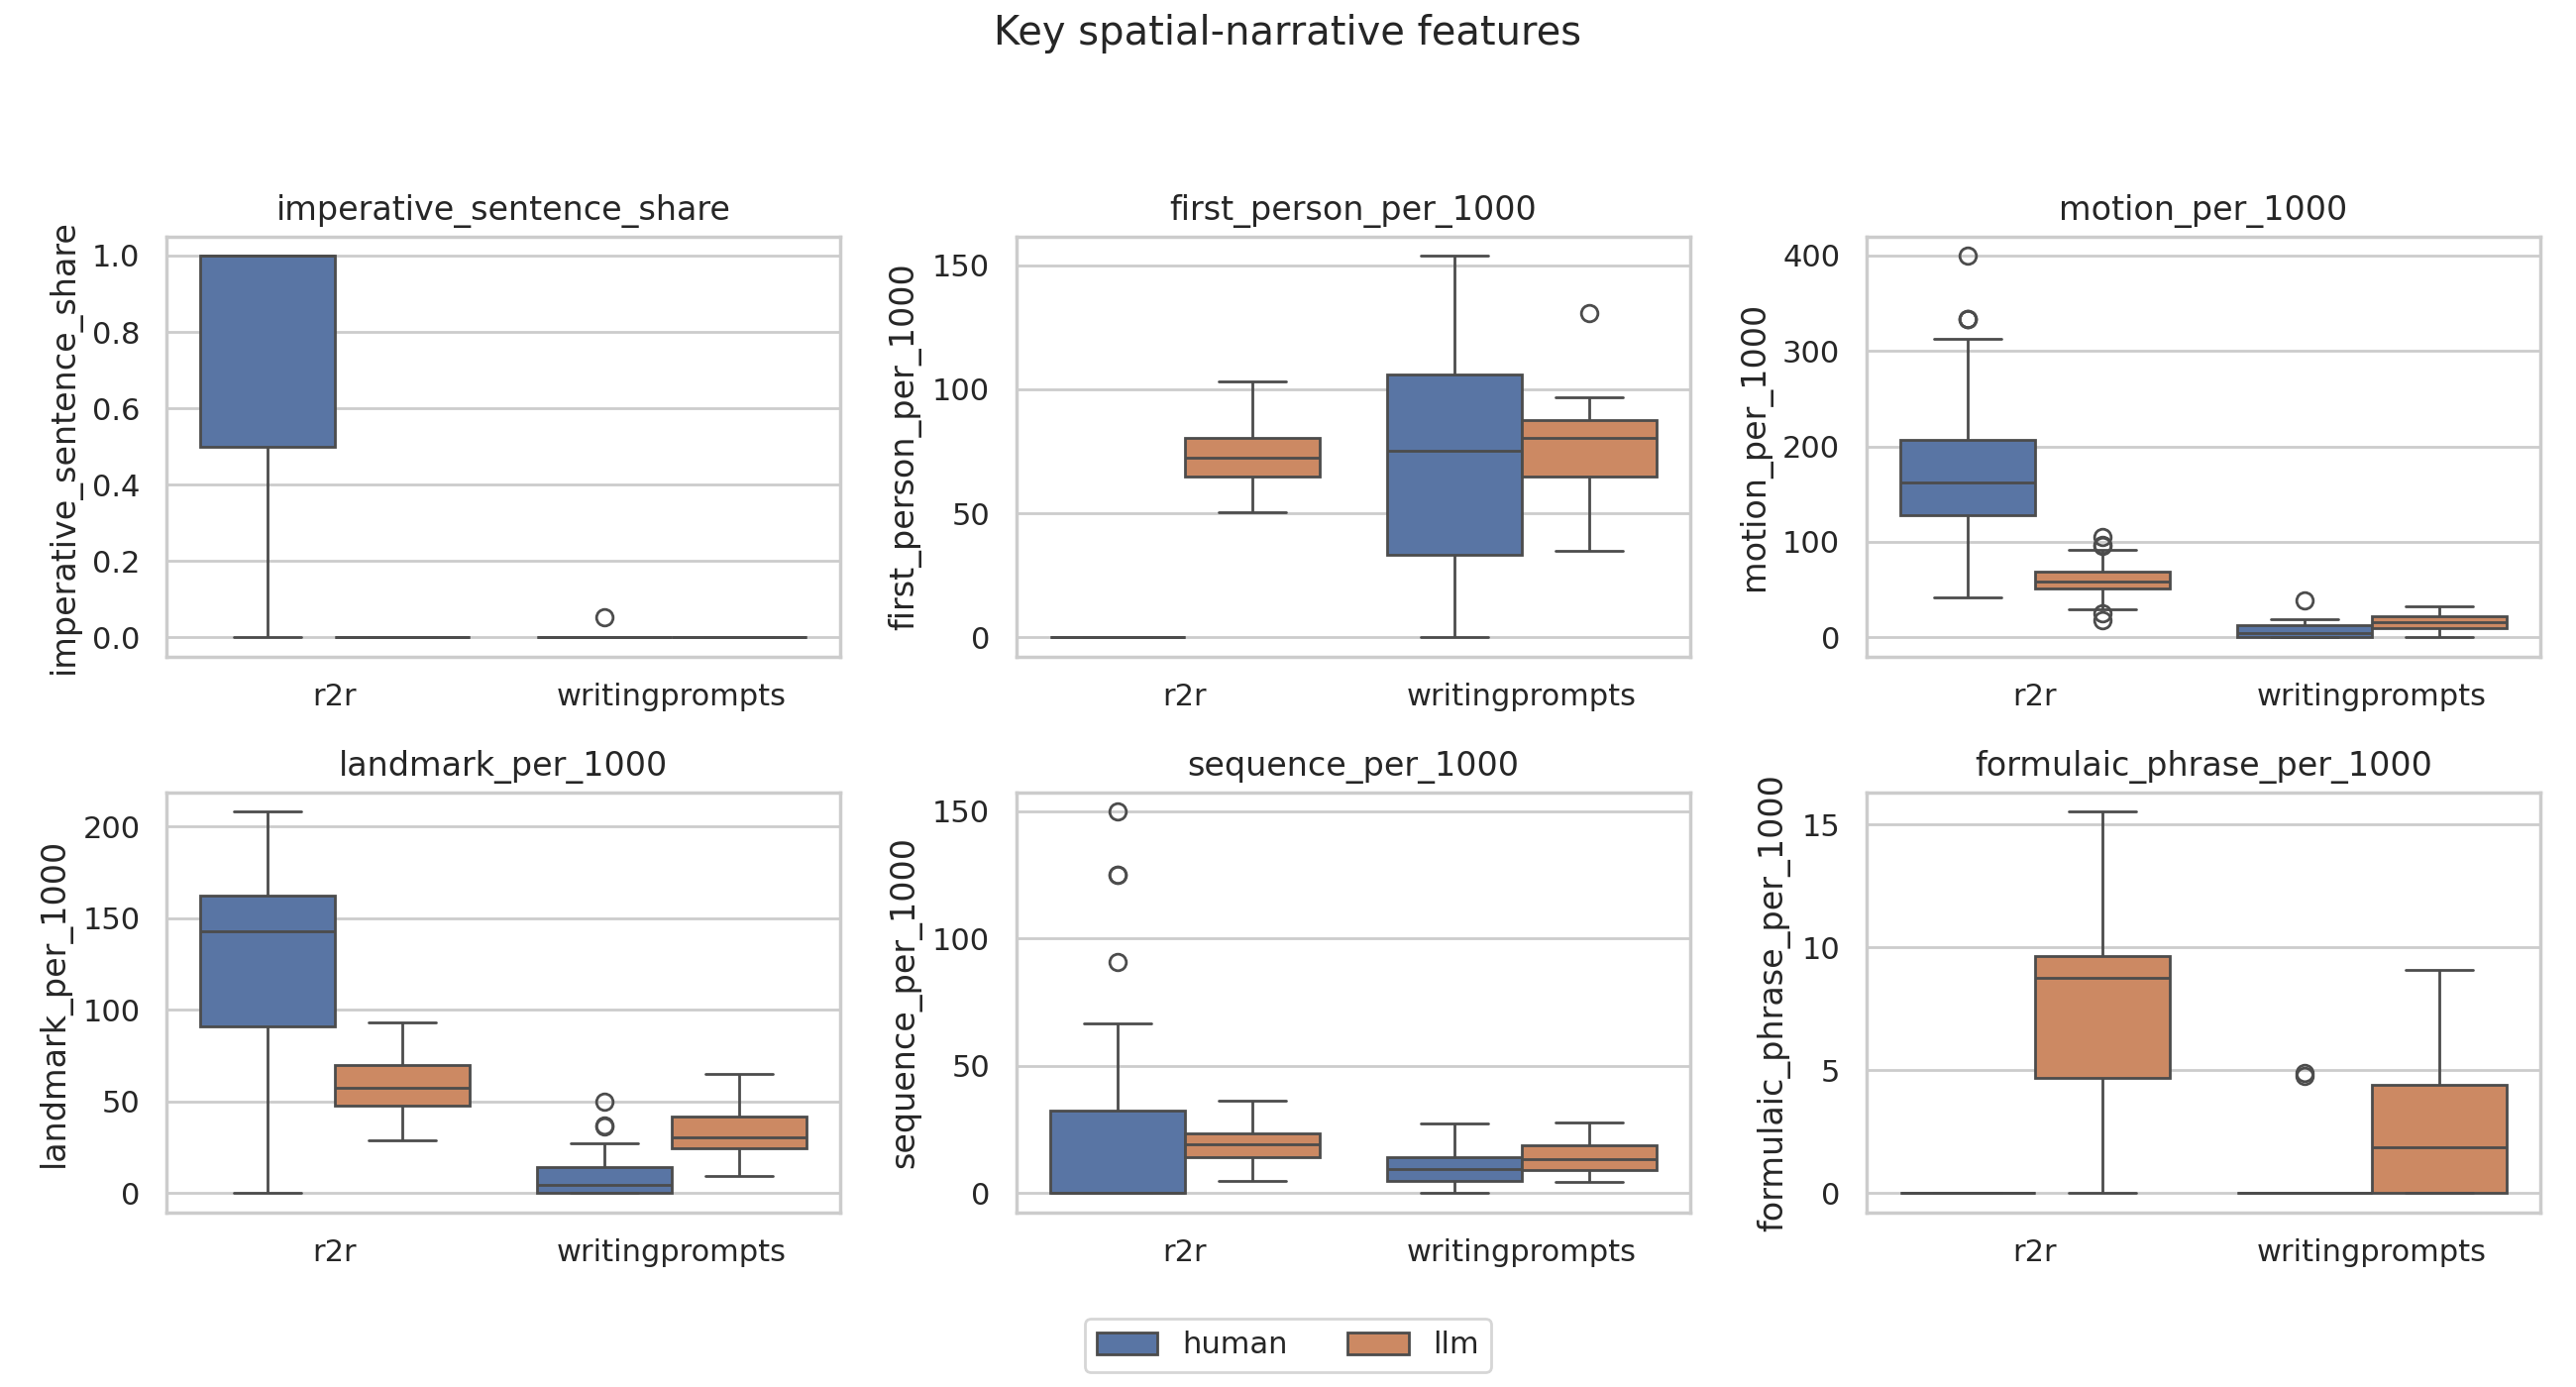
\includegraphics[width=0.95\linewidth]{figures/key_feature_distributions.png}
    \caption{Distributions for selected spatial and narrative features. \gptmini outputs concentrate on sensory and formulaic scene language, while human \rtr instructions contain more task-directed imperative structure.}
    \label{fig:key-feature-distributions}
\end{figure}

\begin{table}[t]
    \centering
    \resizebox{\textwidth}{!}{%
    \begin{tabular}{@{}lrrlr@{}}
        \toprule
        \textbf{Feature} & \textbf{Human mean} & \textbf{\llm mean} & \textbf{Direction} & \textbf{BH $q$} \\
        \midrule
        \texttt{landmark\_per\_1000} & 9.79 & 32.92 & \llm higher & $4.62{\times}10^{-8}$ \\
        \texttt{sensory\_per\_1000} & 5.93 & 16.75 & \llm higher & $1.19{\times}10^{-7}$ \\
        \texttt{route\_step\_density} & 43.55 & 64.90 & \llm higher & $8.33{\times}10^{-6}$ \\
        \texttt{motion\_per\_1000} & 7.81 & 16.92 & \llm higher & $7.06{\times}10^{-5}$ \\
        \texttt{formulaic\_phrase\_per\_1000} & 0.28 & 2.79 & \llm higher & $1.96{\times}10^{-4}$ \\
        \texttt{survey\_route\_ratio} & 0.289 & 0.117 & \llm lower & $5.60{\times}10^{-4}$ \\
        \bottomrule
    \end{tabular}}
    \caption{Key feature differences within the \writingprompts prose-control subset. Both human and \llm texts are prose, yet \gptmini still uses more landmarks, movement language, sensory detail, and formulaic phrasing.}
    \label{tab:writingprompts-features}
\end{table}


The \writingprompts feature table is the strongest evidence against a pure route-instruction explanation. In this prose-control subset, \gptmini uses more landmarks (32.92 vs. 9.79 per 1,000, $q=4.62{\times}10^{-8}$), more sensory language (16.75 vs. 5.93 per 1,000, $q=1.19{\times}10^{-7}$), more route-step language (64.90 vs. 43.55, $q=8.33{\times}10^{-6}$), and more motion verbs (16.92 vs. 7.81 per 1,000, $q=7.06{\times}10^{-5}$). The model also has a lower survey/route ratio, suggesting a preference for embodied path progression over map-like description.

\subsection{Feature Importance and External Transfer}
\label{sec:importance-results}

\begin{table}[t]
    \centering
    \begin{tabular}{@{}lr@{}}
        \toprule
        \textbf{Feature} & \textbf{Coefficient} \\
        \midrule
        \texttt{first\_person\_per\_1000} & 1.463 \\
        \texttt{word\_count} & 1.434 \\
        \texttt{hapax\_ratio} & 1.217 \\
        \texttt{formulaic\_phrase\_per\_1000} & 1.089 \\
        \texttt{sensory\_per\_1000} & 0.991 \\
        \texttt{landmark\_reuse\_ratio} & 0.972 \\
        \texttt{survey\_route\_ratio} & -0.896 \\
        \texttt{dialogue\_mark\_density} & -0.860 \\
        \texttt{sentence\_count} & -0.845 \\
        \texttt{narrative\_route\_ratio} & -0.835 \\
        \bottomrule
    \end{tabular}
    \caption{Top standardized logistic coefficients for predicting \llm authorship. Positive coefficients are \llm-leaning and negative coefficients are human-leaning.}
    \label{tab:top-coefficients}
\end{table}


\Figref{fig:top-coefficients} and \tabref{tab:top-coefficients} show standardized logistic coefficients for predicting \llm authorship. The top positive coefficients are first-person terms, word count, hapax ratio, formulaic phrases, sensory terms, and landmark reuse. The strongest negative coefficients include survey/route ratio, dialogue mark density, sentence count, and narrative/route ratio. The model is therefore not separating author class by a single feature; it combines perspective, style, route structure, and repetition.

\begin{figure}[t]
    \centering
    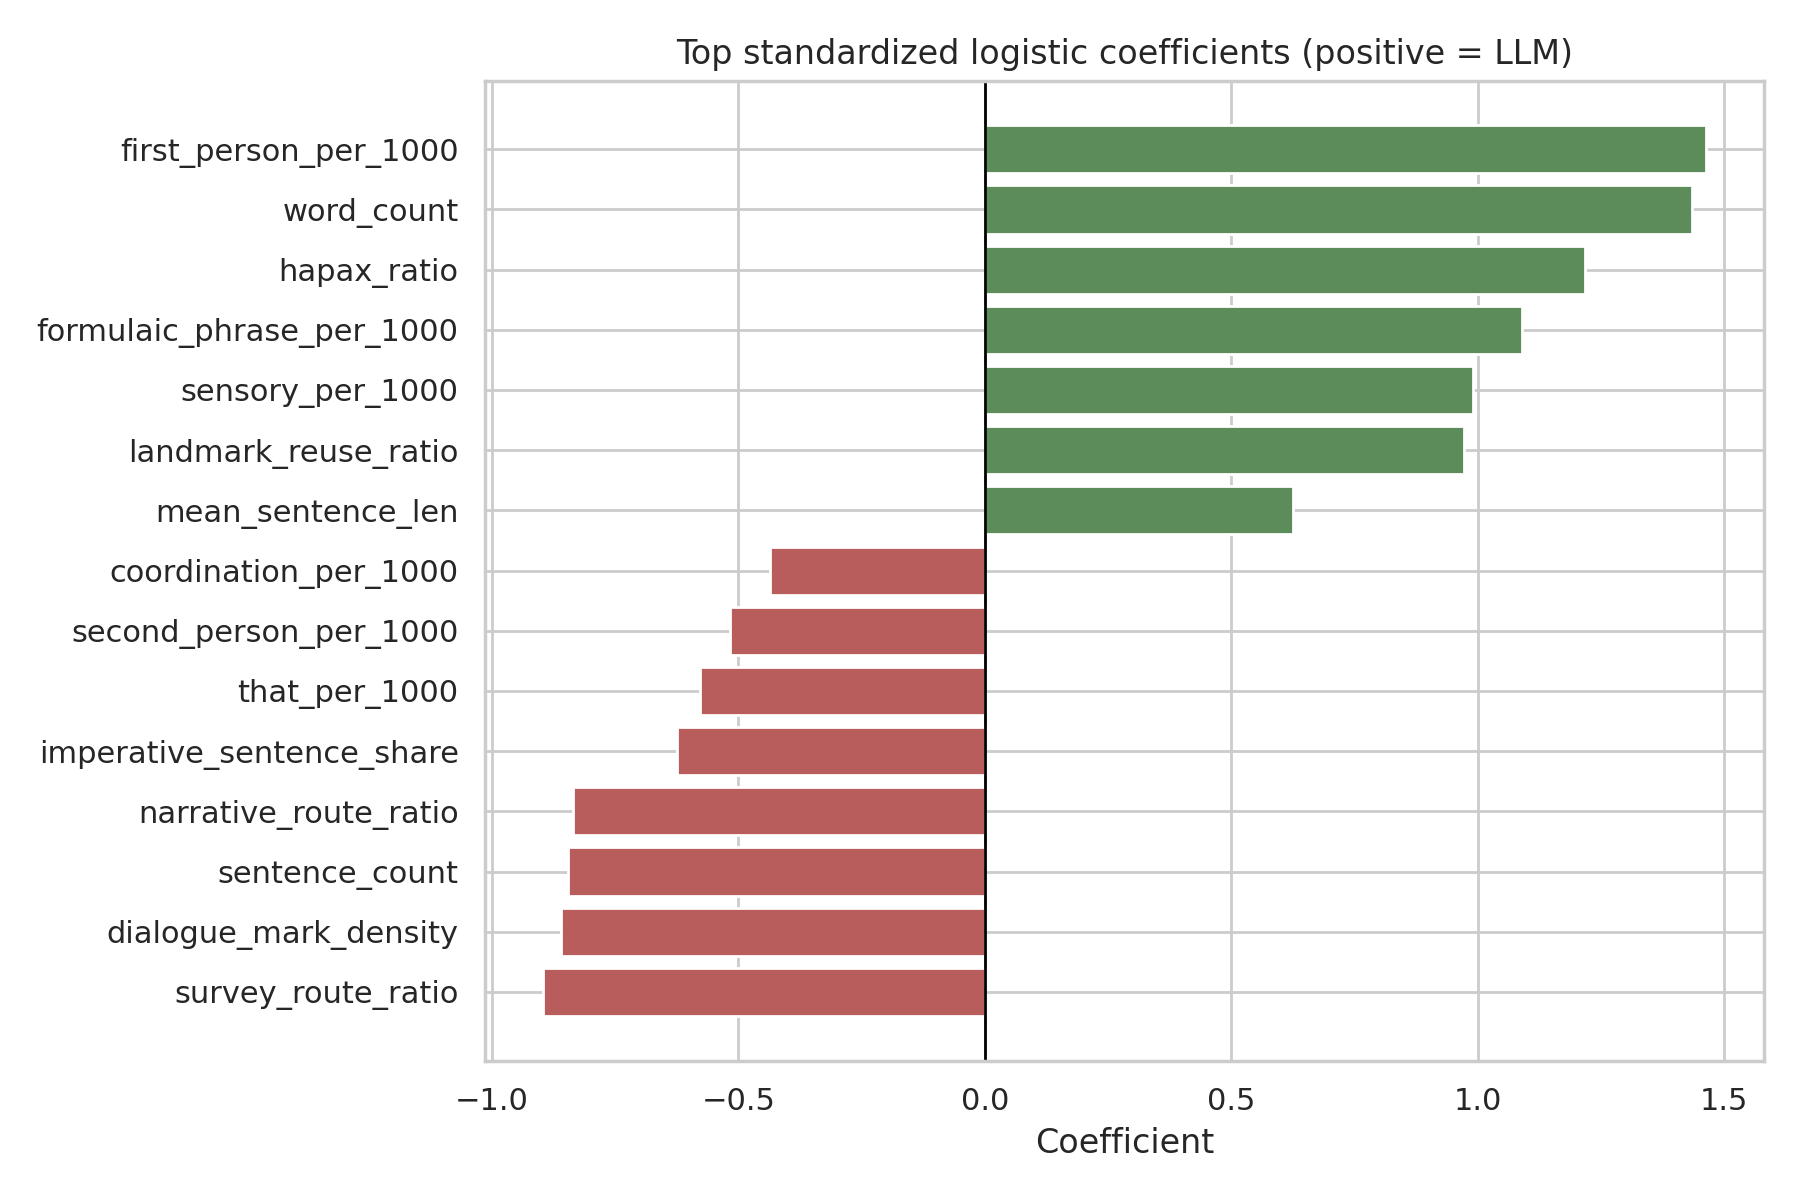
\includegraphics[width=0.85\linewidth]{figures/top_logistic_coefficients.png}
    \caption{Top standardized logistic-regression coefficients for predicting \llm authorship. Positive coefficients are \llm-leaning; negative coefficients are human-leaning.}
    \label{fig:top-coefficients}
\end{figure}

The \longstory sanity check shows limited transfer. A classifier trained on the main corpus predicts 43.8\% of the 80 \longstory excerpts as \llm, with mean \llm probability 0.412. This weak external transfer suggests that the measured fingerprint is not simply ``any AI story.'' It is tied to the tested model, prompts, corpus mixture, and spatial-navigation setup.
